\documentclass[a4paper]{article}

%% Language and font encodings
\usepackage[french]{babel}
\usepackage[utf8]{inputenc}
\usepackage[T1]{fontenc}

\usepackage{float}

\setlength{\parindent}{1em}
%\setlength{\parskip}{1ex plus 0.5ex minus 0.2ex}
\newcommand{\hsp}{\hspace{20pt}}
\newcommand{\HRule}{\rule{\linewidth}{0.5mm}}

\usepackage{algorithm}
\usepackage[noend]{algpseudocode}
\algnewcommand{\algorithmicand}{\textbf{ and }}
\algnewcommand{\algorithmicor}{\textbf{ or }}
\algnewcommand{\OR}{\algorithmicor}
\algnewcommand{\AND}{\algorithmicand}
\algnewcommand\algorithmicforeach{\textbf{for each}}
\algdef{S}[FOR]{ForEach}[1]{\algorithmicforeach\ #1\ \algorithmicdo}
\newcommand{\myfrac}[2]{\frac{\displaystyle {#1}}{\displaystyle {#2}}}

%% Sets page size and margins
\usepackage[a4paper,top=3cm,bottom=2cm,left=3cm,right=3cm,marginparwidth=1.75cm]{geometry}

%% Useful packages
\usepackage{amsmath}
\usepackage{amssymb}
\usepackage{graphicx}
\usepackage{subcaption}
\usepackage[colorinlistoftodos]{todonotes}
\usepackage[colorlinks=true, allcolors=blue]{hyperref}
\usepackage{graphicx}

\usepackage{enumitem}

\usepackage{listings}
\lstset{language=Python} 

\usepackage[htt]{hyphenat}

%% equations
\usepackage{amsthm}
\usepackage[retainorgcmds]{IEEEtrantools}

%% theorem and proposition
\newtheorem{prop}{Proposition}
\newtheorem*{prop*}{Proposition}
\newtheorem{thm}{Théorème}

\newenvironment{myproof}[1][\proofname]{\proof[#1]\mbox{}\\*}{\endproof}

%% references shortcuts (Arthur) 
\usepackage{suffix}
\renewcommand{\eqref}[1]{équation~\ref{#1}}
\newcommand{\algoref}[1]{algorithme~\ref{#1}}
\newcommand{\figref}[1]{figure~\ref{#1}}
\newcommand{\tabref}[1]{tableau~\ref{#1}}
\newcommand{\secref}[1]{section~\ref{#1}}
\newcommand{\probref}[1]{problème~\ref{#1}}
\newcommand{\propref}[1]{proposition~\ref{#1}}
\newcommand{\theoremref}[1]{théorème~\ref{#1}}
\newcommand{\chapref}[1]{chapitre~\ref{#1}}
\newcommand{\appref}[1]{annexe~\ref{#1}}
\WithSuffix\newcommand\algoref*[1]{algorithme~\ref{#1} p.~\pageref{#1}}
\WithSuffix\newcommand\figref*[1]{figure~\ref{#1} p.~\pageref{#1}}
\WithSuffix\newcommand\eqref*[1]{équation~\ref{#1} p.~\pageref{#1}}
\WithSuffix\newcommand\tabref*[1]{tableau~\ref{#1} p.~\pageref{#1}}
\WithSuffix\newcommand\secref*[1]{section~\ref{#1} p.~\pageref{#1}}
\WithSuffix\newcommand\probref*[1]{problème~\ref{#1} p.~\pageref{#1}}
\WithSuffix\newcommand\propref*[1]{proposition~\ref{#1} p.~\pageref{#1}}
\WithSuffix\newcommand\chapref*[1]{chapitre~\ref{#1} p.~\pageref{#1}}

\usepackage[backend=biber,uniquename=init,giveninits=true,
             %% "et al" pour > deux auteurs, & pour exactement 2
             uniquelist=false,maxcitenames=2,mincitenames=1,maxbibnames=99,
             isbn=false,url=false,doi=false,bibstyle=numeric
]{biblatex}
\addbibresource{references.bib}


\begin{document}

\begin{titlepage}
  \begin{center}

      \makebox[0.5\textwidth][c]{%
        
\includegraphics[width=0.33\textwidth]{images/sorbonne.png}%
    }%

    \vspace{4cm}
    % Title
    \HRule \\[0.4cm]
    { \huge \bfseries Twitter et les sondages automatiques\\[0.4cm] }

      \textsc{\LARGE Rapport du projet DAC}\\[0.4cm]

    \HRule \\[0.4cm]

    % Author and supervisor
    \begin{minipage}{0.4\textwidth}
      \begin{flushleft} \large
        Kim-Anh Laura \textsc{Nguyen}\\
        Arij \textsc{Riabi}\\
        Promo DAC 2018-2019 \\
      \end{flushleft}
    \end{minipage}
    \begin{minipage}{0.5\textwidth}
      \begin{flushright} \large
          \emph{Encadrants :} Vincent \textsc{Guigue} \\
          Nicolas \textsc{Baskiotis}\\
      \end{flushright}
    \end{minipage}

      \vspace{2cm}

  \end{center}
  %\end{sffamily}
\end{titlepage}
%\maketitle

\newpage

\tableofcontents

\newpage

\section{Introduction}

\newpage

\section{Analyse de sentiments et transfert}

\newpage

\section{Analyse de communautés}

Dans l'objectif d'extraire des communautés d'utilisateurs favorables à un
candidat en particulier , nous considérons désormais une approche axée, non pas
sur le contenu des tweets, mais sur les liens entre utilisateurs. Nous
souhaitons donc construire un graphe de communautés basé sur les interactions
entre utilisateurs, i.e., un graphe où chaque nœud correspond à un utilisateur
et chaque arc désigne un retweet, une citation ou une réponse. Nous utilisons la
bibliothèque Python networkx \cite{networkx}, spécialisée dans l'étude des
graphes et des réseaux.

L'algorithme de partitionnement que nous utilisons est la méthode de Louvain
\cite{blondel-louvain}, qui permet d'extraire les communautés de réseaux en
optimisant la modularité, i.e., la densité d'arêtes à l'intérieur des
communautés comparée à celle des arêtes reliant les communautés entre elles. 

\begin{figure}[H]
	\center 
	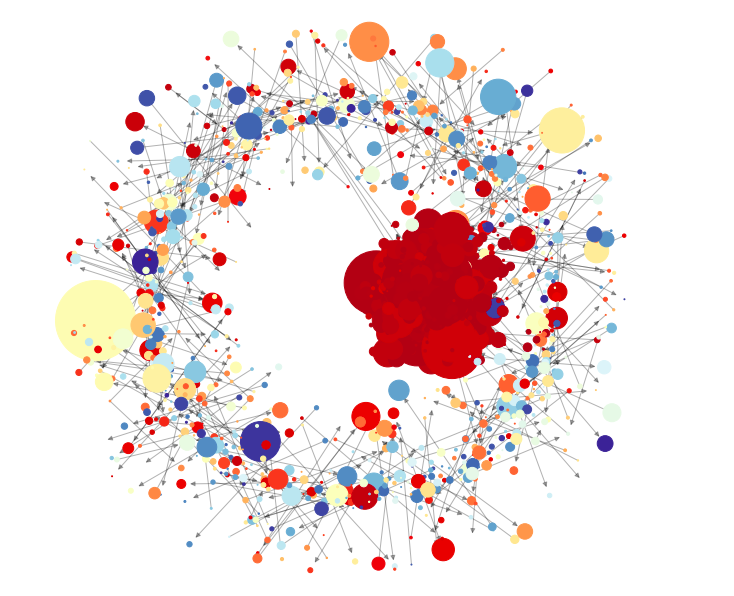
\includegraphics[width=0.9\textwidth]{images/analyse_communautes/communautes_total.png}
    \caption{Graphe de communautés construit sur 10000 tweets}
    \label{img:communautes-total}
\end{figure}

La \figref{img:communautes-total} contient le graphe de communautés construit à
partir d'un échantillon de 10000 tweets. Cette partition contient plus de 700
communautés, et nombreuses sont celles ne contenant très peu d'utilisateurs
(moins de 100) pour être significatives : nous 

Nous décidons donc de garder uniquement les communautés de plus de 100 nœuds.




\newpage

\section{Fusion des deux approches}

\newpage

\section{Conclusion}

\printbibliography
\end{document}
